\documentclass[../main.tex]{subfiles}

\begin{document}

\section{Empirical Results}
\label{sec: Empirical Results}

This chapter describes the results of the experiment.
Section~\ref{sub: Model Verification} verifies whether the model assumed in Section~\ref{sub: Model} is applicable even to actual inflation forecasts.
Section~\ref{sub: Forecast Accuracy} describes the forecast accuracy of each forecasting methods, and Section~\ref{sub: Parameter Estimation} contains the estimated parameter values in the ensembles.
We confirm the behavior of the proposed human-machine ensemble method in the real problem in Section~\ref{sub: Behavior of Human-Machine Ensemble}.
Finally, Section~\ref{sub: Summary and Interpretations} summarizes the results and interpret them.

\subsection{Model Verification}
\label{sub: Model Verification}

\begin{figure}
  \centering
  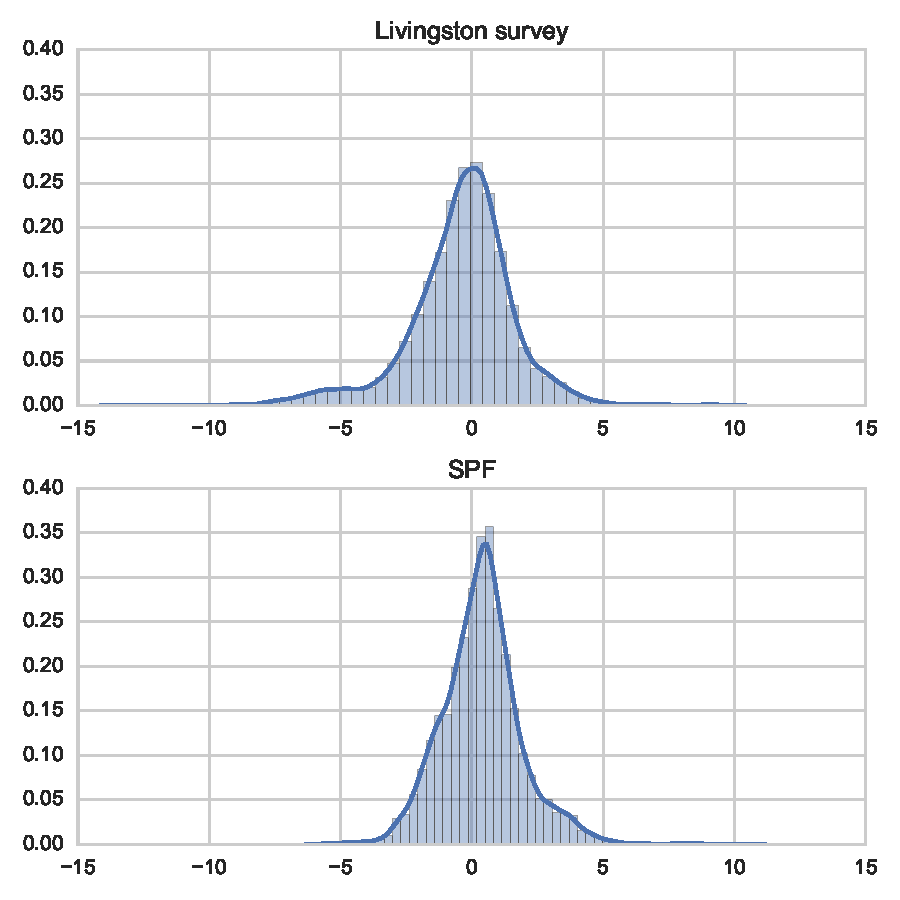
\includegraphics[width=0.9\textwidth]{results-error_distribution.pdf}
  \caption{
    Distributions of individual errors in the Livingston Survey and the SPF when forecasting annual CPI change rate.
    The numbers of samples are 5258 and 4706, and the means are -0.40 and 0.37, respectively.
  }\label{fig: error distribution}
\end{figure}

We assumed that the forecast errors by humans are unbiased, that is, the average forecast error is $0$ in Section~\ref{ssub: Humans model}.
Figure~\ref{fig: error distribution} shows the error distributions when the individuals forecast the annual CPI change rate.
The upper side is the Livingston Survey, and the lower side is the SPF\@.
The figure indicate that the errors of individuals are distributed around zero equally.
The means of these distributions are $-0.40$ in the Livingston Survey and $0.37$ in the SPF\@.

\begin{figure}
  \centering
  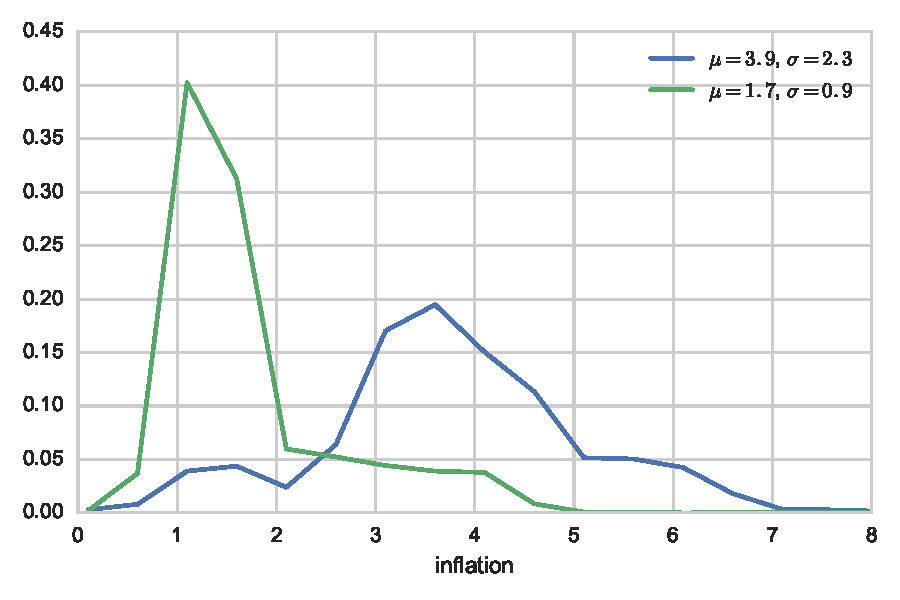
\includegraphics[width=0.9\textwidth]{results-machine_outputs.pdf}
  \caption{
    Examples of distributions outputted by the RNN models.
  }\label{fig: machine outputs}
\end{figure}

\begin{figure}
  \centering
  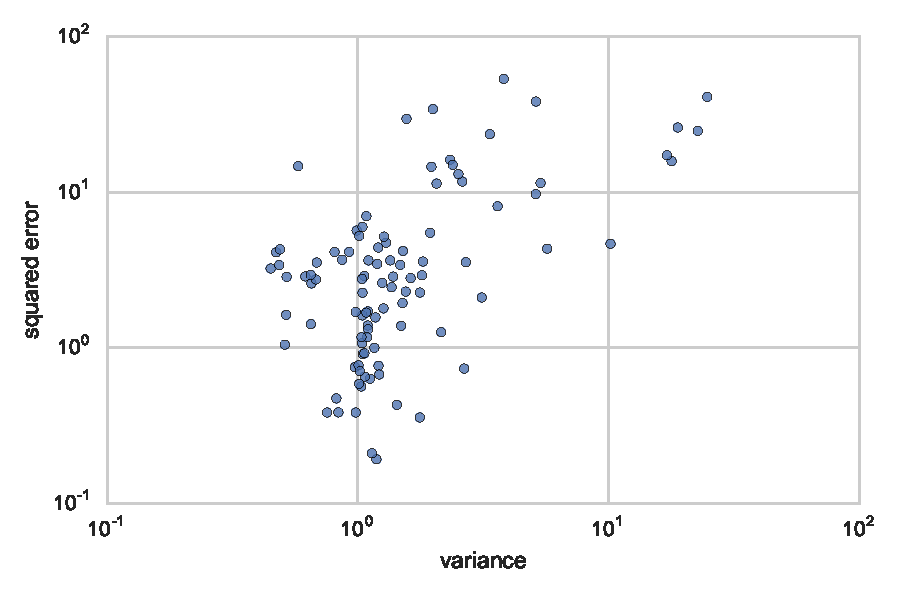
\includegraphics[width=0.9\textwidth]{results-var_sqerr.pdf}
  \caption{
    Relationship between the variances of the ditributions outputted by the RNN model and the actual squared errors in the test set.
  }\label{fig: var-sqerr}
\end{figure}

We also assumed that the machine outputs can be regarded as posterior distributions of the target value.
Figure~\ref{fig: machine outputs} shows examples of the discrete probability distributions actually outputted by the RNN model that forecast the annual CPI change rate.
Since the model learned the training set, this distribution is applicable to the training set well, but to what extent it applies to the test set depends on its generalization ability.
However, when applying the human-machine ensemble method, we consider the distributions are reliable, and regard the variance as the expected squared error.
Therefore, we examined the relationship between the variance of the distribution outputted by the model and the actual squared error.
Figure~\ref{fig: var-sqerr} plots those relationships in the test set.
Although there are variations, it is considered to be correlated.

\subsection{Forecast Accuracy}
\label{sub: Forecast Accuracy}

\begin{table}[t]
  \caption{
    Relative RMSEs of each forecasting method in the test set.
    Bold entries are the smallest RMSEs in each column.
  }\label{tab: forecast accuracy}
  \begin{center}
    \small
    \begin{tabular}{lrrrrrrr}
\toprule
{} &  CPI-LIV &  CPI-SPF &  CoreCPI &    PCE &  CorePCE &  CPI-6M &  CPI-1998 \\
\midrule
ARMA     &    1.000 &    1.000 &    1.000 &  1.000 &    1.000 &   1.000 &     1.000 \\
RNN      &    0.889 &    0.889 &    0.788 &  0.933 &    0.842 &   1.010 &     0.941 \\
survey   &    0.704 &\textbf{0.736}&\textbf{0.767}&\textbf{0.711}&    0.848 &   0.939 &     0.940 \\
ensemble &\textbf{0.689}&\textbf{0.736}&\textbf{0.767}&  0.724 &\textbf{0.827}&\textbf{0.931} &\textbf{0.755} \\
\bottomrule
\end{tabular}

  \end{center}
\end{table}

Table~\ref{tab: forecast accuracy} shows the relative RMSEs for the test set of each forecasting method.
Each entry reports the ratio of its RMSE to the RMSE of the benchmark, ARMA(1,1).
That is, if the value is smaller than 1, it is more accurate than the benchmark, and otherwise, it is less accurate than the benchmark.

Most of the values in the row of RNN were less than 1, that is, the RNN models made more accurate forecasts than ARMA(1,1) overall.
However, the RNN model that forecasted 6 months CPI change was less accurate than ARMA(1,1).
This suggests that ARMA(1,1) is better for shorter term inflation forecasts than RNN, as mentioned in the past study~\cite{Nakamura2005}.

The average forecasts of five people sampled from the surveys outperformed the benchmark in all cases.
And the survey was the most accurate in forecasting PCE\@.
In comparison with RNN, the surveys made more accurate forecasts except for CorePCE\@.
While the RNN models make forecasts based only on the past 12 months sequences, humans can include various information such as economic conditions in the forecasts.
This is why the surveys were more accurate than other models.

The ensembles made the most accurate forecasts in 4 out of 7 cases.
In other two cases, CPI-SPF and CoreCPI, the RMSEs were the same as the surveys, and it was the best score.
This is because the variances outputted by the RNN models were larger than $\covh$ of the SPF, and the ensembles always selected to use humans only.

\subsection{Parameter Estimation}
\label{sub: Parameter Estimation}

\begin{table}
  \caption{
    Parameter values of each ensemble estimated from the training set.
  }\label{tab: parameters}
  \begin{center}
    \small
    \begin{tabular}{lrrrrrrr}
\toprule
{} &  CPI-LIV &  CPI-SPF &  CoreCPI &    PCE &  CorePCE &  CPI-6M &  CPI-1998 \\
\midrule
$\varh$  &    2.869 &    1.887 &    1.379 &  1.453 &    1.134 &   0.986 &     2.952 \\
$\covh$  &    1.846 &    0.873 &    0.455 &  0.450 &    0.168 &   0.652 &     1.924 \\
$\covmh$ &    1.772 &    1.096 &    0.668 &  0.510 &    0.056 &   0.497 &     1.821 \\
\bottomrule
\end{tabular}

  \end{center}
\end{table}

Table~\ref{tab: parameters} shows the parameters $\varh$,$\covh$ and $\covmh$ of each ensemble.
They were estimated from the training set.
$\varh$ is the average variance of the individual errors in a survey; $\covh$ is the average covariance in errors of an arbitrary human pair; $\covmh$ is the average covariance in the errors of a RNN model and an arbitrary human.
The smaller $\varh$, the higher the ability of individuals in the group; the smaller $\covh$, the more diverse the group; the smaller $\covmh$, the more different the forecasts of humans and machine.

The row of $\varh$ shows that the values of CPI-LIV and CPI-1998 were large.
CPI-LIV and CPI-1998 forecasted the annual CPI change rate usigng the Livingston Survey as the forecasts of humans.
CPI-6M had the small $\varh$ as it forecasted shorter period, 6 months.
The $\varh$ of the ensembles that used the SPF were smaller than CPI-LIV\@.
In particular, the values of CoreCPI and CorePCE were small.
This suggests that it is easier to forecast indexes that excludes food and energy.

Next, let us look at $\covh$ and $\covmh$.
In CPI-LIV, CorePCE, CPI-6M and CPI-1998, where the ensembles performed well, $\covmh$ was smaller than $\covh$.
That is, the forecasts of humans and machines were more diverse than that of only humans.
On the other hand, in CPI-SPF, CoreCPI and PCE, where the ensemble did not perform well, $\covmh$ was larger than $\covh$.
This means that adding a machine to a group of humans does not increase the diversity of forecasts.

\subsection{Behavior of Human-Machine Ensemble}
\label{sub: Behavior of Human-Machine Ensemble}

As described in Section~\ref{sub: Overview}, the basic idea of the human-machine ensemble method is that when the machine receives a pattern not in the past and outputs large variance, the ensemble combines forecasts of humans.
This section confirms whether the human-machine ensemble method behaves as expected through CPI-LIV\@.

\begin{figure}
  \centering
  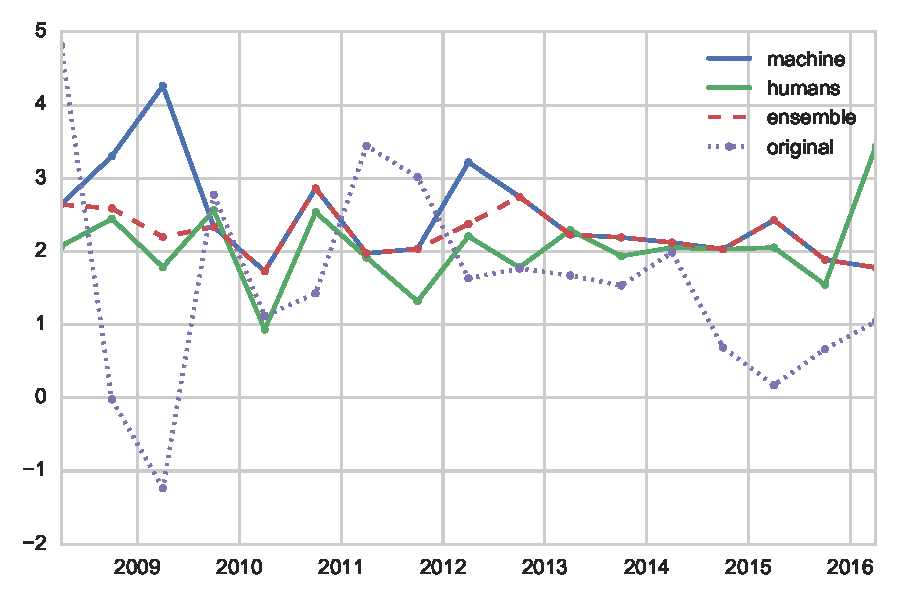
\includegraphics[width=\textwidth]{results-behavior.pdf}
  \caption{
    Behavior of the ensemble CPI-LIV in the test set.
    The purple dotted line shows the actual inflation; the blue line shows the forecasts of the RNN model; the green line shows the average forecasts of five people randomly sampled from the Livingston Survey; and the red dotted line shows the forecasts of the ensemble.
  }\label{fig: behavior}
\end{figure}

Figure~\ref{fig: behavior} is a line graph that shows the annual CPI change rate and the forecasts of the RNN model, the Livingston survey and the ensemble in the test set.
The dotted purple line represents the actual inflation, so the closer to this means the forecast is accurate.
The blue line shows the forecasts of the RNN model, and the green is forecasts using the Livingston Survey.
The forecasts of the ensemble is the red line.
When the ensemble used the machine only or humans only, the line overlaps each line.

In the test set, the period from 2008 to 2009 is applicable to the assumed scenario.
From the end of 2007 to 2009 was global financial crisis triggered by the subprime mortgage.
Particularly, the Bankruptcy of Lehman Brothers in September 2008 decreased the index levels of CPI and PCE\@.
In the training set from 1957 to 2007, the annual CPI change rate never took a negative value, so it is the pattern not in the past.
In fact, the forecasts of the RNN model in December 2008 and June 2009 were largely out.
However, at this time the forecast of the ensemble depended on forecasts of humans rather than the forecasts of machine.
In other words, the ensemble emphasized forecasts of humans because the machine received patterns that were not in the past and outputted distributions with large variances.

\begin{table}[p]
  \caption{
    Behavior of the ensemble CPI-LIV in the test set.
    From the left, the columns show the squared errors of the RNN model, the variances outputted by the RNN model, the numbers of humans the ensemble employed, and the squared errors of the ensemble.
  }\label{tab: behavior}
  \begin{center}
    \begin{tabular}{lrrrr}
\toprule
{} &  machine error &  variance &  n &  ensemble error \\
\midrule
Jun 2008 &           4.74 &      1.53 &  0 &            4.74 \\
Dec 2008 &          11.06 &      2.15 &  5 &            6.81 \\
Jun 2009 &          30.23 &      2.81 &  5 &           11.80 \\
Dec 2009 &           0.19 &      1.63 &  0 &            0.19 \\
Jun 2010 &           0.38 &      0.90 &  0 &            0.38 \\
Dec 2010 &           2.06 &      1.72 &  0 &            2.06 \\
Jun 2011 &           2.16 &      1.15 &  0 &            2.16 \\
Dec 2011 &           0.96 &      1.22 &  0 &            0.96 \\
Jun 2012 &           2.51 &      2.12 &  5 &            0.55 \\
Dec 2012 &           0.96 &      1.65 &  0 &            0.96 \\
Jun 2013 &           0.31 &      1.35 &  0 &            0.31 \\
Dec 2013 &           0.43 &      1.33 &  0 &            0.43 \\
Jun 2014 &           0.02 &      1.28 &  0 &            0.02 \\
Dec 2014 &           1.81 &      1.21 &  0 &            1.81 \\
Jun 2015 &           5.08 &      1.45 &  0 &            5.08 \\
Dec 2015 &           1.49 &      1.07 &  0 &            1.49 \\
Jun 2016 &           0.55 &      0.96 &  0 &            0.55 \\
\bottomrule
\end{tabular}

  \end{center}
\end{table}

Table~\ref{tab: behavior} shows the squared error and variance of each forecast of the RNN model, the number of humans and the squared error of each forecast of the ensemble CPI-LIV in the test set.
This table also suggests that there is a correlation between variances and squared errors of machine forecasts since when a variance is large, the squared error is also large.
In addition, when the variance was large, the ensemble adopted many human forecasts and reduced the error.

Basically, the ensemble behaved as expected, but the number of humans $n$ can only take $0$ or $N_{\max} = 5$.
This is because the ensemble parameters shown in Table~\ref{tab: parameters} did not satisfy the condition (\ref{eq: condition}), which is for having a local minimum.
If this condition is not satisfied, the optimal $n$ is $0$ or $N_{\max}$, as in the two graphs in the lower side of Figure~\ref{fig: graph of ensemble}.

The reason why equation (\ref{eq: condition}) is not satisfied is that humans and a machine do not make so different forecasts.
The index level at the time of forecasting has a great influence on forecasts both of humans and machines.
For example, if the inflation rate at the time of forecasting is 1\%, both of humans and machines will forecast around 1\% as annual inflation, and when these forecasts goes out, both humans and machines take a similar error.
Thus, $\covmh$ can not take a sufficiently small value for $\varh$ and $\covh$, and can not satisfy the equation (\ref{eq: condition}).

\subsection{Summary and Interpretations}
\label{sub: Summary and Interpretations}

As a result of model verification, the models proposed in Section~\ref{sub: Model} are applicable to actual inflation forecasts.
The mean error of individuals in the Livingston Survey and the SPF was about $0$, and there was no bias in the distributions.
Thus, the proposed human model, where forecasts of humans are unbiased, is valid.
Additionally, the variances outputted by the machine and the squared errors in the test set were distributed approximately along a line with a slope of 1 passing through the origin.
Hence, it is possible to create a prediction model that performs as the proposed machine model, which outputs probability distributions of which variance is regarded as expected squared error.

We compared forecast accuracy of the proposed human-machine ensemble method with other forecasting methods.
The ensembles made the most accurate forecasts in 4 out of 7 cases.
In other two cases, the ensembles used forecasts of only humans, so the scores were the same as the survey forecasts.
In the last case, the forecasts of the ensemble were less accurate than the survey forecasts, but were more accurate than ARMA(1,1) and RNN\@.

As a reason why the proposed ensemble method did not work well in 3 out of 7, it is suggested that $\covmh$ was greater than $\covh$.
In other words, adding a machine to a group of humans did not increase the diversity, and did not reduce the error.

The three cases CPI-SPF, CoreCPI and PCE, where the ensemble method did not perform well, used the SPF as forecasts of humans.
Since the SPF began from 1981, its sample period is shorter than the Livingston Survey.
This implies that estimation of the parameters $\covmh$ and $\covh$ did not work well.

Finally, we assumed the human-machine ensemble method takes the advantage of humans forecasts when the expected error of the machine is large as shown in Figure~\ref{fig: schematic}.
Therefore, we verified the behavior of an ensemble after the Bankruptcy of Lehman Brothers.
As a result, the ensemble adopted human forecasts as expected, and reduced the error.

\end{document}
